\documentclass[a4paper, 10pt, final, garamond]{book}
\usepackage{cours-preambule}
\graphicspath{{./figures/}}

\makeatletter
\renewcommand{\@chapapp}{Contr\^ole de connaissances}
\makeatother

\toggletrue{student}
% \HideSolutionstrue
% \toggletrue{corrige}
\renewcommand{\mycol}{black}

\begin{document}
\setcounter{chapter}{9}

\chapter{Électrocinétique en RSF \ifstudent{ (12')}}

\begin{enumerate}[label=\sqenumi]
	\nitem{1}%
	Convertir les signaux suivants en complexes sous la forme «~amplitude complexe
	$\times$ exponentielle temporelle~»~:
	\begin{DispWithArrows*}[format=rLlCl]
		e(t) = E_0\cos(\wt)
		\quad & ; \quad
		s(t) = S\cos(\wt + \f)
		\quad & ; \quad
		u(t) = U\sin(\wt)
		\\
		\wsw{
			\eu(t) = E_0\exr^{\jwt}
		}
		\quad & ; \quad
		\wsw{
			\xul{s}(t) = S\exr^{\jj (\wt+\f)} = \xul{S}\exr^{\jwt}
		}
		\quad & ; \quad
		\wsw{
			\uu(t) = U\exr^{\jj (\wt - \frac{\pi}{2})} = \Uu\exr^{\jwt}
		}
		\\
		&
		\wsw{
			\qav \xul{S} = S\exr^{\jj \f}
		}
		&
		\wsw{
			\qav \Uu = U\exr^{-\jj \frac{\pi}{2}}
		}
	\end{DispWithArrows*}
	\nitem{2}%
	Donner et démontrer la relation du pont diviseur de tension pour
	deux impédances $\Zu_1$ et $\Zu_2$ en série d'une part, et en parallèle
	d'autre part.\\
	\begin{isd}[]
		\begin{center}
			\sswitch{
				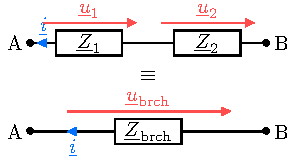
\includegraphics[height=3cm, draft=true]{zserie}
			}{
				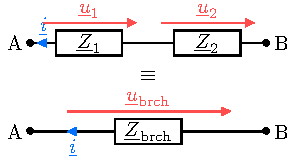
\includegraphics[height=3cm]{zserie}
			}
			\captionof{figure}{Association série}
		\end{center}
		\wsw{
			\[
				\Iu = \frac{\Uu}{\Zu\ind{brch}} = \frac{\Uu_k}{\Zu_k}
				\Lra
				\boxed{
					\Uu_k = \frac{\Zu_k}{\Zu\ind{brch}}\Uu\ind{brch}
				}
			\]
		}
		\tcblower
		\begin{center}
			\sswitch{
				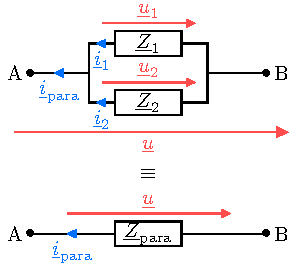
\includegraphics[height=3cm, draft=true]{zpara}
			}{
				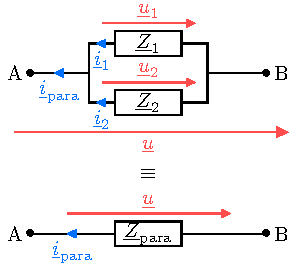
\includegraphics[height=3cm]{zpara}
			}
			\captionof{figure}{Association parallèle}
		\end{center}
		\wsw{
			\[
				\Uu = \Zu\ind{para}\Iu\ind{para} = \Zu_1\Iu_1
				\Lra
				\boxed{
					\Iu_k = \frac{\Zu\ind{para}}{\Zu_k}\Iu\ind{para}
				}
			\]
		}
	\end{isd}
	\nitem{3}%
	% \noindent
	\begin{minipage}[t]{.65\linewidth}
		Pour un système excité par un signal d'entrée $e(t) = E_0\cos(\wt)$,
		indiquer ce qu'est le RSF et la forme réelle des signaux de sortie $s(t)$.
		Application au circuit RC série en RSF~: transformez-le en RSF, puis
		déterminer $\Uu_C(\w)$ \textbf{par un pont diviseur de tension} et en
		déduire $U_C(\w)$ et $\f_C(\w)$.
	\end{minipage}
	\hfill
	\begin{minipage}[t]{.30\linewidth}
		\vspace{-12pt}
		\begin{center}
			\sswitch{
				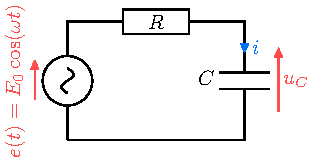
\includegraphics[width=.8\linewidth]{rc_rsf}
			}{
				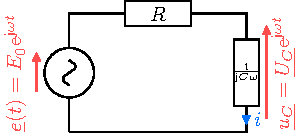
\includegraphics[width=.8\linewidth]{rc_rsf-cplx}
			}
			\vspace{-10pt}
			\captionof{figure}{RC en RSF.}
		\end{center}
	\end{minipage}
	\\
	\wsw{
		Le régime sinusoïdal forcé correspond au régime temporel pour lequel le
		système est décrit par la solution \textbf{particulière} de son équation
		différentielle, après que la solution homogène soit nulle. On suppose alors
		\[
			s(t) = S\cos(\wt + \f)
		\]
		Sur le RC série, on applique un PdT sur les amplitudes complexes~:
		\begin{gather*}
			\Uu_C =
			\frac{\frac{1}{\jcw}}{R + \frac{1}{\jcw}}E_0 =
			\frac{1}{1 + \jj RC\w}E_0
			% \Ra
			\\\Ra
			U_C = \abs{\Uu_C}
			\Lra
			\boxed{
				U_C = \frac{E_0}{\sqrt{1+(RC\w)^2}}
			}
			\Ra
			% \\\Ra
			\f_C = \arg{\Uu_C}
			\Lra
			\boxed{
				\f_C = -\arctan(RC\w)
			}
			\quad \text{car} \Re(\arg(1 + \jj RC\w)) > 0
		\end{gather*}
	}
	\nitem{4}%
	Définir ce qu'est la résonance avec vos propres mots. Citer sans détailler un
	exemple du quotidien \textbf{autre que la balançoire}. Indiquer comment se
	définit mathématiquement la résonance pour un système, et définissez
	mathématiquement ce qu'est la bande passante en donnant les mots de
	vocabulaire nécessaires et à l'aide d'un schéma.
	\smallbreak
	\begin{isd}[righthand ratio=.3]
		\wsw{
			La résonance correspond au fait d'apporter de l'énergie à un système
			oscillant à une fréquence qui permet l'addition de ces deux énergies.
			Exemple~: instrument à vent. Avec $X(\w)$ l'amplitude réel du signal
			excité, on a
			\begin{align*}
				\text{résonance}
				\quad & \Lra \quad
				\exists \w_r \neq (0,+\infty)~:~ X(\w_r) = X_{\max}
				\\
				\text{bande passante}
				\quad & \triangleq \quad
				\{\w ~|~ X(\w) > X_{\max}/\sqrt{2}\}
			\end{align*}
			\begin{itemize}
				\item $\w_1$ et $\w_2$ les \textbf{pulsations de coupure}~;
				\item $\D\w = \abs{\w_2 - \w_1}$ la \textbf{bande passante}~;
				\item $\w_r/\D\w$ l'\textbf{acuité de la résonance}.
			\end{itemize}
		}
		\vspace{-15pt}
		\tcblower
		\begin{center}
			\sswitch{
				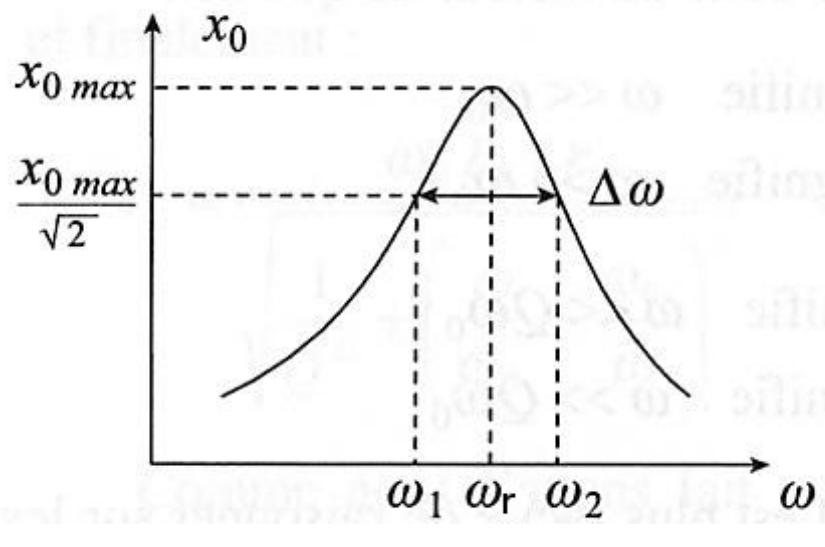
\includegraphics[width=\linewidth, draft=true]{bandepass_moche}
			}{
				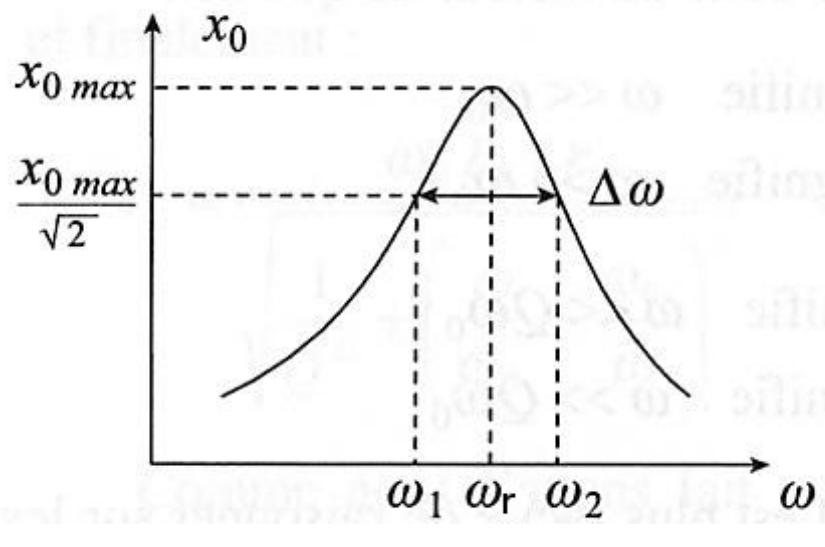
\includegraphics[width=\linewidth]{bandepass_moche}
			}
			\vspace{-15pt}
			\captionof{figure}{Bande passante}
		\end{center}
	\end{isd}
	\vspace*{-30pt}
	\ifstudent{
		\begin{tikzpicture}[remember picture, overlay]
			\node[anchor=north west, align=left]
			at ([shift={(1.4cm,0)}]current page.north west)
			{\\[5pt]\Large\bfseries Nom~:\\[10pt]\Large\bfseries Prénom~:};
			\node[anchor=north east, align=right]
			at ([shift={(-1.5cm,-17pt)}]current page.north east)
			{\Large\bfseries Note~:\hspace{1cm}/10};
		\end{tikzpicture}
	}
\end{enumerate}
\end{document}
